%\documentclass[a4paper,landscape, 5pt]{article}
\documentclass[10pt]{article}
\usepackage[a4paper, margin=0.1in, landscape]{geometry}
%\usepackage{graphicx} % Required for inserting images
\usepackage{graphicx}
\usepackage{multicol}
\usepackage{xcolor}
\usepackage{amsfonts}
\usepackage{wrapfig}
\usepackage{amsmath}  % For various math symbols and 
\usepackage{amssymb}  % For additional math symbols
\usepackage{bm}       % For bold math symbols

\usepackage{lipsum}

\usepackage[compact]{titlesec}
% Change title spacing
\titlespacing{\section}{0pt}{*0}{*0}
\titlespacing{\subsection}{0pt}{*0}{*0}
\titlespacing{\subsubsection}{0pt}{*0}{*0}

% Change title color
% \newcommand{\sectionnewcolor}[1]{%
%     \definecolor{section_color}{rgb}{#1}%
%     \titleformat*{\section}{\normalfont\normalsize\bfseries\color{section_color}}%
%     \titleformat*{\subsection}{\normalfont\normalsize\bfseries\color{section_color}}%
%     \titleformat*{\subsubsection}{\normalfont\normalsize\bfseries\color{section_color}}%
% }
\definecolor{default_section_color}{rgb}{0,0,0} % Default color
\newcounter{colornumber}
\setcounter{colornumber}{1}
\newcommand{\sectionnewcolor}{%
    \ifcase\thecolornumber%
        \colorlet{section_color}{red}%
    \or
        \colorlet{section_color}{green}%
    \or
        \colorlet{section_color}{blue}%
    \or
        \colorlet{section_color}{cyan}%
    \or
        \colorlet{section_color}{magenta}%
    \or
        \colorlet{section_color}{yellow}%
    \or
        \colorlet{section_color}{orange}%
    \or
        \colorlet{section_color}{purple}%
    \or
        \colorlet{section_color}{teal}%
    \or
        \colorlet{section_color}{lime}%
    \or
        \colorlet{section_color}{pink}%
    \or
        \colorlet{section_color}{brown}%
    \or
        \colorlet{section_color}{indigo}%
    \or
        \colorlet{section_color}{turquoise}%
    \or
        \colorlet{section_color}{gold}%
    \or
        \colorlet{section_color}{silver}%
    \or
        \colorlet{section_color}{slategray}%
    \or
        \colorlet{section_color}{olive}%
    \or
        \colorlet{section_color}{maroon}%
    \else
        \colorlet{section_color}{default_section_color}%
    \fi
    
    \titleformat*{\section}{\normalfont\normalsize\bfseries\color{section_color}}%
    \titleformat*{\subsection}{\normalfont\normalsize\bfseries\color{section_color}}%
    \titleformat*{\subsubsection}{\normalfont\normalsize\bfseries\color{section_color}}%
    \stepcounter{colornumber}%
}

\newcommand{\sectiondivider}{%
    \vspace{4pt}%
    \hrule%
    \vspace{4pt}%
}

% Change text spacing
\setlength{\parindent}{0pt}
\setlength{\columnseprule}{0.2pt}
\setlength{\intextsep}{0pt}%
% \setlength{\columnsep}{7pt}%

\begin{document}

\begin{multicols*}{4}

\sectionnewcolor
\section*{Regression}
\subsection*{Terminology}

- Data consists of \textbf{pairs} ($\mathbf{x}_n$, $y_n$), where $y_n$ is the n’th output and $x_n$ is a vector of $D$ inputs. The number of pairs $N$ is the data-size and $D$ is the dimensionality.

- Two goals of regression: \textbf{prediction} and \textbf{interpretation}

- The regression function: $y_{n}\approx f_w(\mathbf{x}_{n})\ \forall n$

- Regression finds correlation not a causal relationship.

- \textbf{Input variables} a.k.a. covariates, independent variables, explanatory variables, exogenous variables, predictors, regressors. 

- \textbf{Output variables} a.k.a. target, label, response, outcome, dependent variable, endogenous variables, measured variable, regressands.

\subsection*{Linear Regression}

- Assumes linear relationship between inputs and output.

- $y_{n}\approx\,f(\mathbf{x}_{n}) :=w_{0}+w_{1}x_{n1}+ ... +w_{D}x_{n D} \\ := \tilde{\bf x}_{n}^{T} \tilde{\bf w}$ contain the additional offset term (\small{a.k.a. bias}).

- Given data we learn the weights $\mathbf{w}$ (\small{a.k.a. estimate or fit the model})

- Overparameterisation $D > N$ eg. univariate linear regression with a single data point $y_{1}\approx w_{0}+w_{1}x_{11}$. This makes the task under-determined (no unique solution).

\subsection*{Loss Functions $\mathcal{L}$}

- A loss function (a.k.a. energy, cost, training objective) quantifies how well the model does (how costly its mistakes are).

- $y \in \mathbb{R} \Rightarrow$ desirable for cost to be symmetric around 0 since $\pm$ errors should be penalized equally.

- Cost function should penalize “large” mistakes and “very large” mistakes similarly to be robust to outliars.

- Mean Squared Error: \\ ${\mathsf{MSE}}(\mathbf{w}):={\frac{1}{N}}\sum_{n=1}^{N}\left[y_{n}-f_{\mathrm{w}}(\mathbf{x}_{n})\right]^{2}$ \\ not robust to outliars.

- Mean Absolute Error: \\ ${\mathsf{MAE}}(\mathbf{w}):={\frac{1}{N}}\sum_{n=1}^{N}|y_{n}-f_{\mathrm{w}}(\mathbf{x}_{n})|$

- Convexity: a function is convex iff a line segment between two points on the function’s graph always lies above the function.

- Convexity: a function $h(\mathbf{u}), \mathbf{u} \in \mathbb{R}^D$ is convex if $\forall \ \mathbf{u}, \mathbf{v} \in \mathbb{R}^D, 0 \leq \lambda \leq  1$: \\ $h(\lambda\mathbf{u}+(1-\lambda)\mathbf{v}) \ \textcolor[RGB]{255,0,0}{\leq} \ \lambda h(\mathbf{u})+(1-\lambda)h(\mathbf{v})$ \\Stirctly convex if $\textcolor[RGB]{255,0,0}{\leq} \Rightarrow \textcolor[RGB]{255,0,0}{<}$ 

- Convexity, a desired computational property:
A strictly convex function has a unique global minimum $\mathbf{w^{*}}$. For convex functions, every local minimum is a global minimum.

- Sums of convex functions are also convex $\Rightarrow$ MSE combined with a linear model is convex in $\mathbf{w}$.

- Proof of convexity for MAE:

\scalebox{0.7}{
$\begin{array}{l}
    {\mathsf{MAE}(\mathbf{w}) := \frac{1}{N} \sum_{n=1}^{N} \mathcal{L}_n(\mathbf{w}), \mathcal{L}_n(\mathbf{w})=|y_{n}-f_{\mathrm{w}}(\mathbf{x}_{n})|} 
    \\ 
    {\mathcal{L}_n(\lambda w_1 + (1-\lambda)w_2) \leq \lambda \mathcal{L}_n(w_1)+(1-\lambda)\mathcal{L}_n(w_2)} 
    \\ 
    {| y_n-x_n^{T}(\lambda w_1 + (1-\lambda)w_2)| \leq \lambda |{y_n-x_n^{T}w_1}| + (1-\lambda)|{y_n-x_n^{T}w_2}|}
    \\
    {(1-\lambda) \geq 0 \Rightarrow (1-\lambda)|{y_n-x_n^{T}w_2}|=|(1-\lambda)y_{n}-(1-\lambda)x_{n}^{T}w_2|}
    \\
    {a=\lambda y_{n}-\lambda x_{n}^{T}w_{1}, b=(1-\lambda)y_{n}-(1-\lambda)x_{n}^{T}w_{2}}
    \\
    {a+b=y_{n}-x_{n}^{T}(\lambda w_{1}+(1-\lambda)w_{2})}
    \\
    {|a + b| \leq |a| + |b| \Rightarrow \mathcal{L}_n(\mathbf{w}) \ \mathsf{convex}\Rightarrow \mathsf{MAE}(\mathbf{w}) \ \mathsf{convex}}
\end{array}$
}

- Huber loss: \\
${\cal H}u b e r(e):=\left\{\begin{array}{l l}{{\frac{1}{2}e^{2}}}&{{,\mathrm{if}\ |e|\leq\delta}}\\ {{\delta|e|-\frac{1}{2}\delta^{2}}}&{{,\mathrm{if}\ |e|>\delta}}\end{array}\right.$ convex, differentiable, and robust to outliers but setting $\delta$ is not easy.

- Tukey’s bisquare loss: \\
$\frac{\partial\mathcal{L}}{\partial e}:=\left\{\begin{array}{l l}{{e\{1-e^{2}/\delta^{2}\}^{2}}}&{{,\mathrm{if}\,\,|e|\leq\delta}}\\ {{0}}&{{,\mathrm{if} \ |e| > \delta}}\end{array}\right.$ non-convex, but robust to outliers.

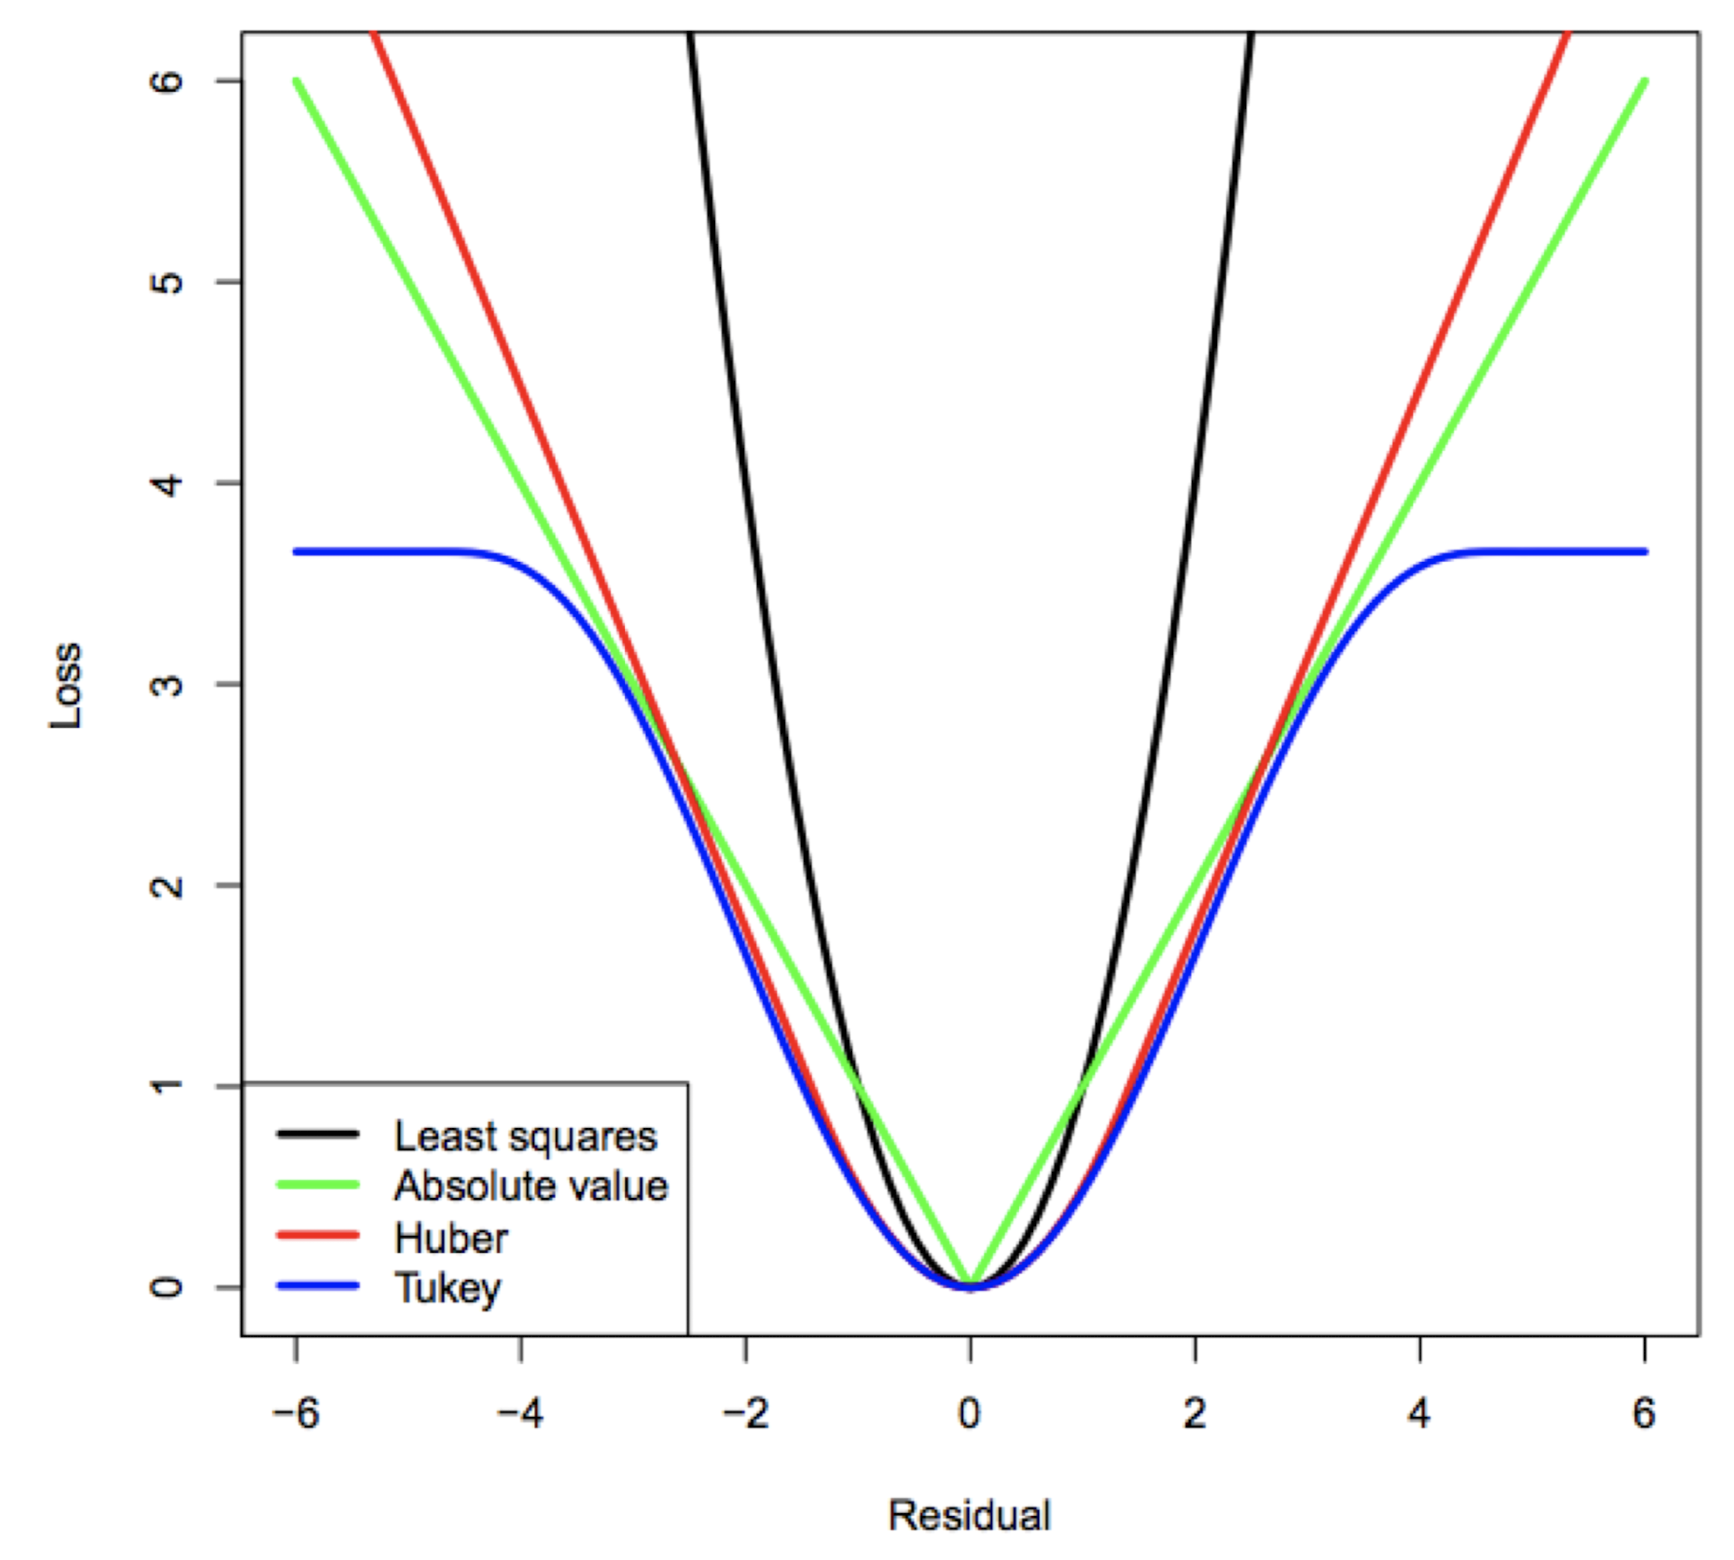
\includegraphics[width=\linewidth]{loss_functions.png}
\sectiondivider

\sectionnewcolor
\section{Optimisation}

- Given $\mathcal{L}(\mathbf{w})$ we want $\mathbf{w^*} \in \mathbb{R}^D$ which minimises the cost: $\min_\mathbf{w} \mathcal{L}(\mathbf{w}) \rightarrow$ formulated as an optimisation problem

- Local minimum $\mathbf{w^*} \Rightarrow \exists \epsilon > 0$ s.t. \\
$\mathcal{L}(\mathbf{w^*}) \leq \mathcal{L}(\mathbf{w}) \ \forall \mathbf{w} \ \mathrm{with} \ \Vert \mathbf{w}-\mathbf{w^*} \Vert < \epsilon$

- Global minimum $\mathbf{w^*}$,
$\mathcal{L}(\mathbf{w^*}) \leq \mathcal{L}(\mathbf{w}) \ \forall \mathbf{w} \in \mathbb{R}^D$

\subsection{Smooth Optimisation}

\vspace{4pt}
\hrule
\vspace{4pt}
\sectiondivider

\sectionnewcolor
\section{Transformers}

% - A transformer is a neural network that iteratively transforms a sequence to another sequence and mixes the information between the sequence elements via self-attention.

% \subsection*{Architecture}


% \begin{wrapfigure}{r}{0.4\columnwidth} 
%     \centering
%     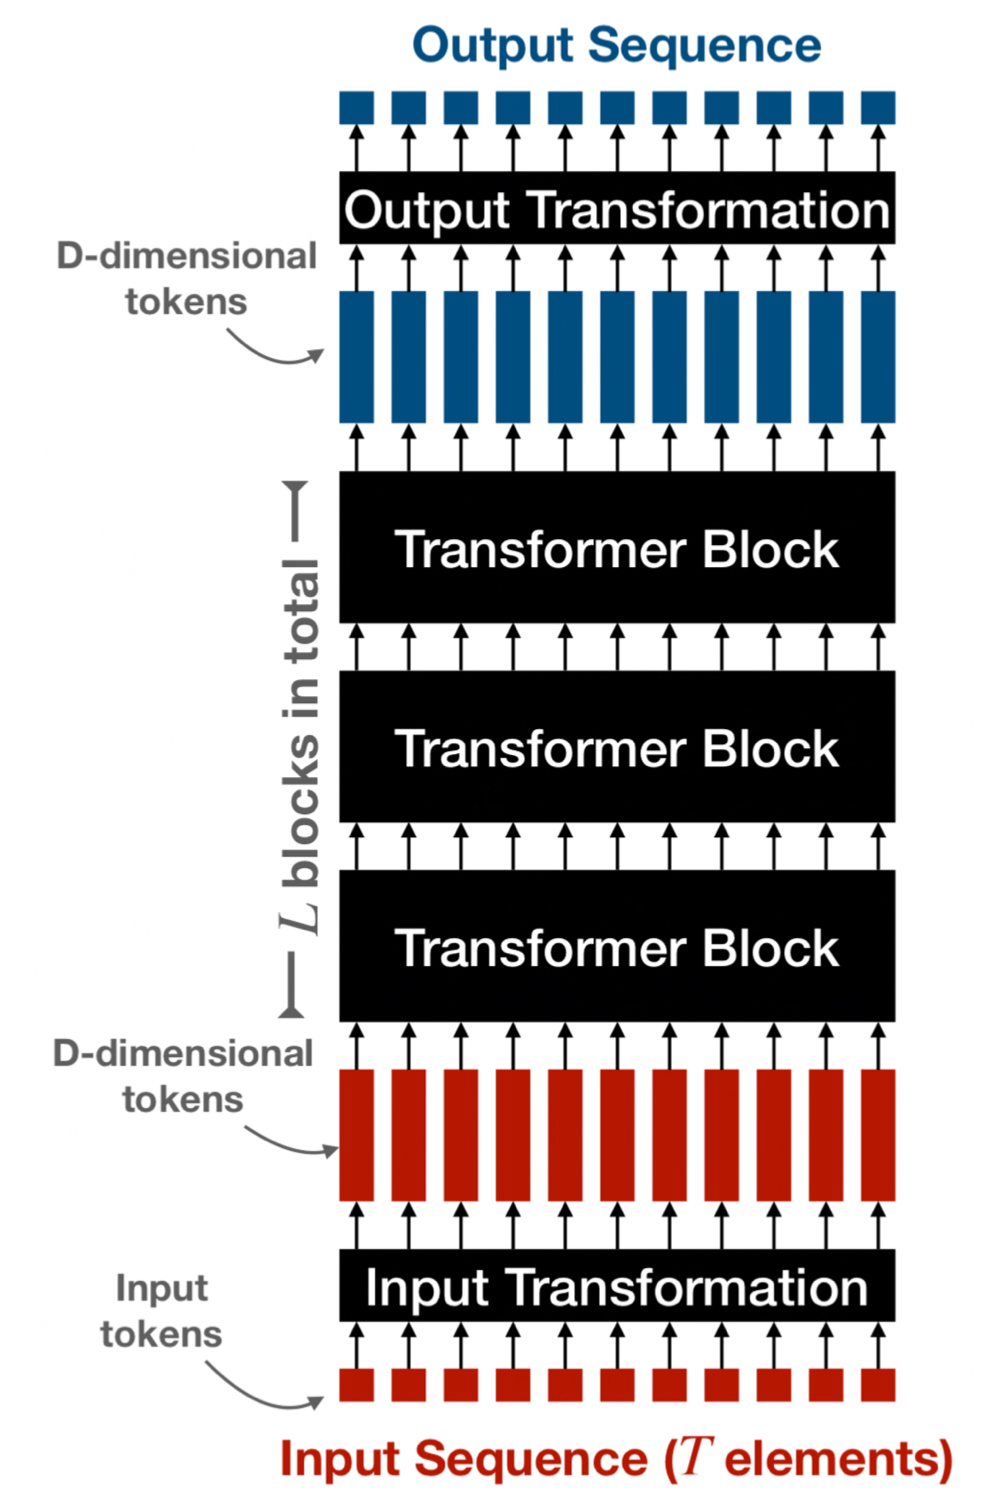
\includegraphics[width=0.4\columnwidth]{figures/transformer_architecture.jpeg}
%     \vspace{-10pt}
% \end{wrapfigure}

- Self-Attention (SA): mixes information between tokens

- Multi-Layer Percep. (MLP): mixes information within each token

- Skip connections are widely used

- Layer normalization (LN) placed at the start of a residual branch

% \begin{wrapfigure}{l}{0.2\columnwidth}
%   % \centering
%   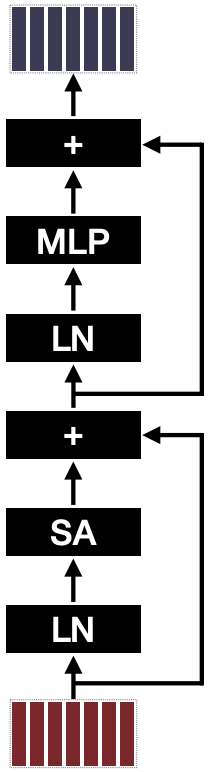
\includegraphics[width=0.2\columnwidth]{figures/transformer_block.png}
% %   \caption{}
% %   \label{fig:cfm_pca2D_wrapped}
% \end{wrapfigure}

\subsection*{Text Token Embeddings}

- Tokenization: split text into sequence of tokens (predefined)

- Convert each token ID $i\in\{1,...,N_{vocab}\}$ into $\mathbf{w}_{i}\in\mathbb{R}^{D}$

- Matrix multiplication $\mathbf{W}\cdot\mathbf{e}_{i}=\mathbf{W}_{:,i}=\mathbf{w}_{i}{\mathrm{~(with~\mathbf{W}\in\mathbb{R}^{D \times N_{vocab}}}})$


- $\mathbf{W}$ learned via backpropagation
% , along with all other transformer parameters (however, the tokenizer procedure is typically fixed in advance and not learned)

- Input sequence of $T$ tokens leads to an input matrix $X\in\mathbb{R}^{T\times D}$

\subsection*{Attention: learning input-dependent weighted average}



% - Attention is a function that transforms a sequence of tokens to a new sequence of tokens using a learned input-dependent weighted average

- Input tokens : $V\in\mathbb{R}^{T_{i n}\times D}$, Output tokens : $Z\in\mathbb{R}^{T_{out}\times D}$

% - Output tokens are simply a weighted average of
% the input tokens:
$z_{i}=\sum_{j=1}^{T_{i}}p_{i j}v_{j}$ i.e. $Z=P V$, Weighting coefficients ${\cal P}\in[0,1]^{T_{out}\times T_{i n}}$ valid probability distributions over input $\textstyle\sum_{j=1}^{T_{i n}}p_{i j}=1$


\begin{wrapfigure}{r}{0.4\columnwidth}
  % \centering
  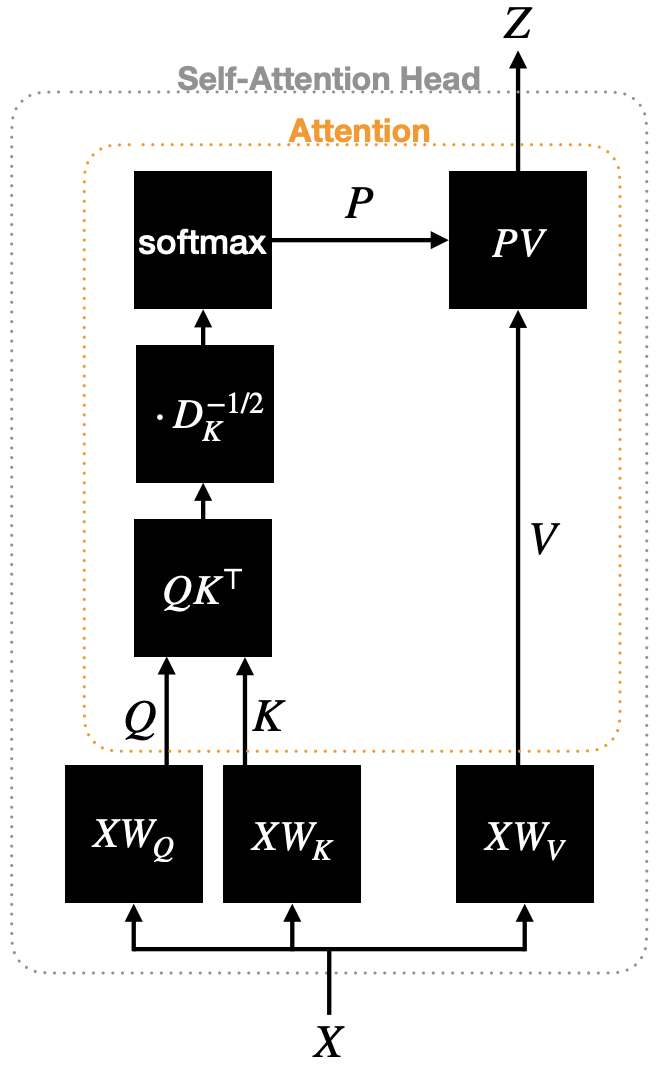
\includegraphics[width=0.4\columnwidth]{figures/self_attention.png}
%   \caption{}
%   \label{fig:cfm_pca2D_wrapped}
\end{wrapfigure}

- Query tokens : $Q\in\mathbb{R}^{T_{out}\times D_{K}}$, Key tokens : $K\in\mathbb{R}^{T_{in}\times D_{K}}$


- Determine weight $p_{i,j}$ based on how simmilar $q_i$ and $k_j$ are.

- Use inner product to obtain raw similarity scores.

- Normalize with softmax (scaled temperature by $\sqrt{D_{K}}$) to obtain a probability distribution. (applied on each row independently)

% - $P=\mathrm{softmax}\left({\frac{Q K^{\mathsf{T}}}{\sqrt{D_{K}}}}\right)$ 
% - The softmax is applied on each row independently. 

- Scaling $\rightarrow$ uniformity at initialization and faster convergence

\subsection*{Self-Attention}



- $V,K,Q$ all derived from same input token
sequence $X\in\mathbb{R}^{T\times D}$

- Values : $V=X W_{V}\in\mathbb{R}^{T\times D},\,W_{V}\in\mathbb{R}^{D\times D}$

- Keys : $K=X W_{K}\in\mathbb{R}^{T\times D_{K}},\,W_{K}\in\mathbb{R}^{D\times D_{K}}$

- Queries : $Q=X W_{Q}\in\mathbb{R}^{T\times D_{K}},W_{Q}\in\mathbb{R}^{D\times D_{K}}$

- $W_{Q},\,W_{V},\,W_{K}$ are learned params.

- $Z=\mathrm{softmax}\left(\frac{X W_{Q}W_{K}^{T}X^{T}}{\sqrt{D_{K}}}\right)X W_{V}$

\subsubsection*{Multi-Head Self-Attention}

% \begin{wrapfigure}{r}{0.3\columnwidth} 
%   \centering
%   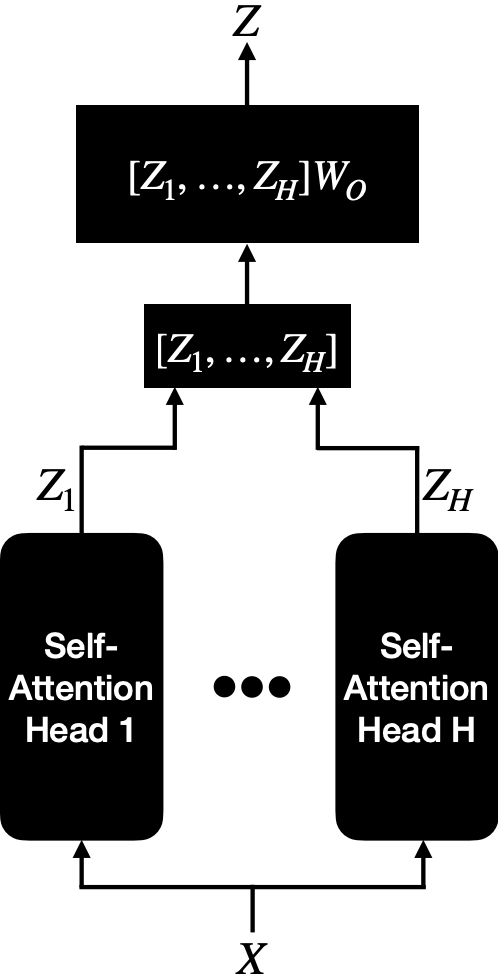
\includegraphics[width=0.3\columnwidth]{figures/multi_head.png}
% \end{wrapfigure}

- Run $H$ Self-Attention “heads” in parallel 
$Z_{h}={\mathrm{softmax}}\left({\frac{X W_{Q,h}W_{K,h}^{\mathsf{T}}X^{\mathsf{T}}}{\sqrt{D_{K}}}}\right)X W_{V,h}\in\mathbb{R}^{T\times D_{V}}$, 
$W_{V,h}\in\mathbb{R}^{D\times D_{V}},\,W_{K,h}\in\mathbb{R}^{D\times D_{K}},\,W_{Q,h}\in\mathbb{R}^{D\times D_{K}}$,
$Z=[Z_{1},\dots,Z_{H}]W_{o}$ where $W_{O}\in\mathbb{R}^{H D_{V}\times D}$ is learned via backprop
% \lipsum[1]

\subsection*{Positional Information}

- Attention by itself does not account for the order of input

- positional encoding in the network $p o s:\left\{1,...,T\right\}\rightarrow\mathbb{R}^{D}$

- e.g. $W_{p o s}$ corresponding to each token's position $t$ to the input embedding. $W_{p o s}\in\mathbb{R}^{D\times T}$ is learned via backprop

\subsection*{MLP: Mixing Information within Tokens}
- Apply the same transformation to each token
independently: $M L P(X)=\varphi(X W_{1})W_{2}$,
$W_{1},W_{2}\in\mathbb{R}^{D\times D}$ learned via backprop

\subsection*{Output Transformations}

% - typically simple: linear transformation or a small MLP

- Single output: transfo. to a special taskspecific input token or to the average tks. Multi outputs: transfo to each token indep.

\subsection*{Vision Transformer Architecture}

% - Self-attention, more general than convolution 

- The receptive field is the whole image after one SA layer

- ViTs require more data than CNNs, reduced inductive bias in extracting local features

- Model attends to image regions semantically relevant for clf

\subsection*{Encoders \& Decoders}

% \begin{wrapfigure}{r}{0.3\columnwidth} 
%   \centering
%   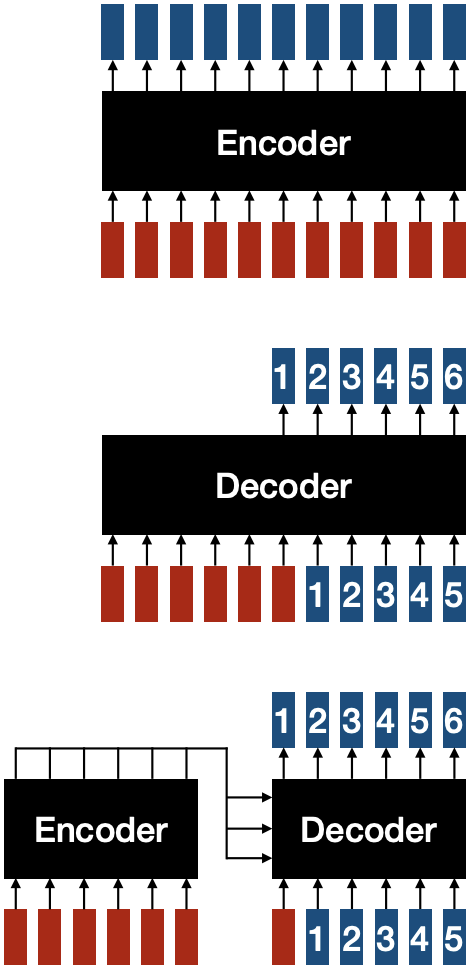
\includegraphics[width=0.3\columnwidth]{figures/encoders_decoders.png}
% \end{wrapfigure}

- Encoders: fixed output size and process all inputs simultaneously

- Decoders: Auto-regressively sample the next token as $x_{t+1}\sim s o f i m a x(f(x_{1},....,x_{t}))$
%  and use it as new input token. Capable of generating responses of arbitrary length.

% - Encoder-decoder (e.g., translation): First encode the whole input (e.g., in one language) and then decode to token by token (e.g., in a different language)

\sectiondivider

\sectionnewcolor
\section*{Adversarial ML}

- We don't understand how NN models generalize and react to shifts in the distribution of data (i.e., distribution shifts)

- Classification problem: $(X,Y)\sim{\mathcal{D}},\;Y$ with range $\{-1,1\}$

- Standard risk: average zero-one loss over $X$: $R(f)=\mathbb{E}_{\mathcal{D}}\left[1_{f(X)\neq Y}\right]=\mathbb{P}_{\mathcal{D}}\left[f(X)\neq Y\right]$ i.e. minimise proba of wrong prediction.


- Adversarial risk: average zero-one loss over small, worst-case perturbations of $X$: $R_{\varepsilon}(f)={{{\mathbb{E}}}}_{\mathcal{D}}\left[\operatorname*{max}_{\hat{x},\|\hat{x}-X\|\leq\varepsilon}1_{f(\hat{x})\neq Y}\right]$

\subsection*{Generating adversarial examples}

- Task: given an input $(x, y)$ and a model $f : \mathcal{X}\rightarrow \{-1,1\}$ find an input $\hat{x}$ s.t.: 
a) $\|{\hat{x}}-x\|\leq\varepsilon$ b) the model $f$ makes a mistake on it.

- Trivial case: x already missclassified $\rightarrow$ no action required

- General case: ${\mathrm{find~}}{\hat{x}}~\mathrm{such~that}{\mathrm{~at}}f({\hat{x}})\neq y\operatorname{and}{\big\vert\vert}{\hat{x}}-x\vert\vert\leq\varepsilon$ i.e. $\hat{x}\in B_{x}(\varepsilon)\cap\{x^{\prime}f(x^{\prime})=-\,y\}$

- Optimization problem with respect to the inputs

- Problem: optimizing the indicator function is difficult: 1) The indicator function $1$ is not continuous 2) The NN prediction $f$ outputs discrete class values $\{-1,1\}$

- Replace the difficult problem involving the indicator with a smooth problem $\operatorname*{max}_{\hat{x},\|\hat{x}-X\|\leq\varepsilon}1_{f(\hat{x})\neq Y} \rightarrow \operatorname*{max}_{\hat{x},\|\hat{x}-X\|\leq\varepsilon}\ell(yg(\hat{x}))$

\begin{wrapfigure}{r}{0.5\columnwidth} 
    \centering
    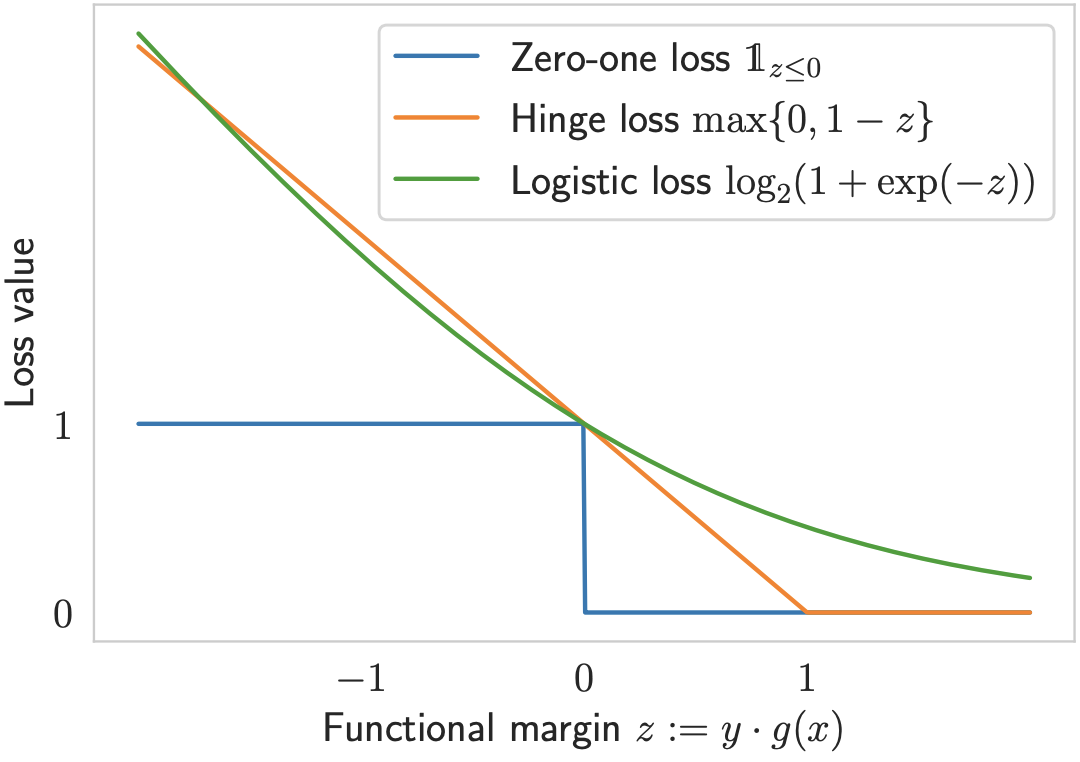
\includegraphics[width=0.5\columnwidth]{figures/classification_losses.png}
\end{wrapfigure}
- decreasing, margin-based (i.e., dependent on $y * g(x)$) classification losses

\subsection*{White-Box attacks}

- Solve $\operatorname*{max}_{\hat{x},\|\hat{x}-X\|\leq\varepsilon}\ell(yg(\hat{x}))$ knowing $g$

- $\nabla_{x}{\ell}(y g(x))=y\ell^{\prime}(y g(x))\,\nabla_{x}g(x)$, with $y\ell^{\prime}(y g(x)) \leq 0$ since classification losses are decreasing.

- Move in direction of $\propto-\,y\,\nabla_{x}g(x)$

- Interpretation $f(x)=\mathrm{{sign}}(g(x))$: If $y=1$ we want to decrease $g(x)$ and follow $-\nabla_{x}g(x)$. If $y=-1$ we want to decrease $g(x)$ and follow $\nabla_{x}g(x)$

- By using $\ell$ and not directly $yg(\hat{x})$ it will extend to multi-class classification and robust training.

- linearize the loss $\tilde{\ell}(x):={\ell}(y g(x))$

$\operatorname*{max}_{\|{\hat{x}}-x\|\leq\varepsilon}{\tilde{\ell}}(x)\\\approx\operatorname*{max}_{\|{\hat{x}}-x\|\leq\varepsilon}{\tilde{\ell}}(x)+\nabla_{x}{\tilde{\ell}}(x)^{T}({\hat{x}}-x) \\={\tilde{\ell}}(x)+\operatorname*{max}_{\|{\hat{x}}-x\|\leq\varepsilon}{\nabla}_{x}{\tilde{\ell}}(x)^{T}({\hat{x}}-x) \\={\tilde{\ell}}(x)+\operatorname*{max}_{\|\delta\|\leq\varepsilon}{\nabla}_{x}{\tilde{\ell}}(x)^{T}{\delta}$

- We need to maximize the inner product under a norm constraint, i.e. find the optimal local update

- This is a simple problem for which we can get a closed-form solution depending on the norm used to measure the perturbation size $||\delta||$

\subsubsection*{One-step attack}

- Solution for the $\ell_2$ norm:

$\delta_{2}^{\star}=\varepsilon\cdot\frac{\nabla_{x}\tilde{\ell}(x)}{||\nabla_{x}\tilde{\ell}(x)||_{2}}=-\;\varepsilon y*\frac{\nabla_{x}g(x)}{||\nabla_{x}g(x)||_{2}} \Rightarrow \\ \hat{x}=x-\varepsilon y\cdot\frac{\nabla_{x}g(x)}{\|\nabla_{x}g(x)\|_{2}}$

- Solution for the $\ell_{\infty}$ norm called \textbf{Fast Gradient Sign Method}:

$\delta_{\infty}^{\star}=\varepsilon\cdot\mathrm{sign}(\nabla_{x}\tilde{\ell}(x))=-\,\varepsilon y\cdot\mathrm{sign}(\nabla_{x}g(x)) \Rightarrow \\ {\hat{x}}=x-\varepsilon y\cdot\operatorname{sign}(\nabla_{x}g(x))$

\subsubsection*{Multi-step attack}


- These updates can be done iteratively and combined with a projection $\Pi$ on the feasible set (i.e., balls $\ell_2$ / $\ell_\infty$ here)

- Projected Gradient Descent (PGD attack)

- $\ell_2$ norm:

$\delta^{t+1}=\Pi_{B_{2}(e)} [\delta^{t}+\alpha\cdot\frac{\nabla\tilde{\ell}(x+\delta^{t})}{\|\nabla\tilde{\ell}(x+\delta^{t})\|_{2}}]$

$\Pi_{B_{2}(\varepsilon)}(\delta)=\left\{\begin{array}{l l}{\varepsilon\cdot\delta/\|\delta\|_{2},\quad{\mathrm{if~}}\|\delta\|_{2}\geq\varepsilon}\\ {\delta \mathrm{~otherwise}}\end{array}\right.$

- $\ell_\infty$ norm:

$\delta^{t+1}=\Pi_{B_{\infty}(\varepsilon)}\left[\delta^{t}+\alpha\cdot\mathrm{sign}(\nabla\tilde{\ell}(x+\delta^{t}))\right],$

$\Pi_{B_{\infty}(\varepsilon)}(\delta)_i=\left\{\begin{array}{l l}{\varepsilon\cdot\mathrm{sign}(\delta_{i}),\ \ \ \mathrm{if}\ |\delta_{i}|\geq\varepsilon}\\ {\delta_i \mathrm{~otherwise}}\end{array}\right.$

- the gradients are computed by backprop w.r.t. inputs, not parameters!

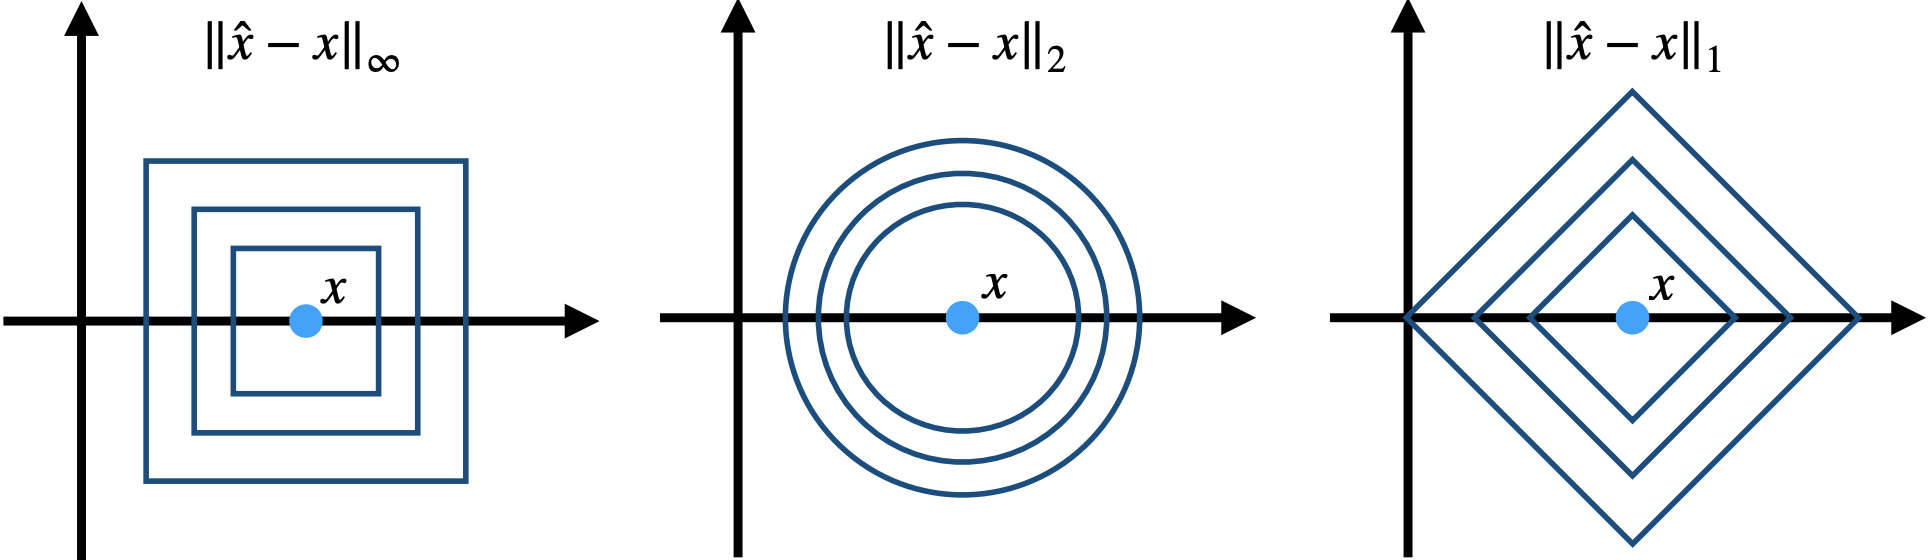
\includegraphics[width=\columnwidth]{figures/lp_norms.png}

\subsection*{Black-box attacks}

- We don't know $g(x)$

- Obtaining a surrogate model can be costly and there is no guarantee of success

- Query-based methods often require a lot of queries (10k-100k), easy to restrict access for the attacker!

\subsubsection*{Query-based gradient estimation}

- Score-based: we can query the continuous model scores $g(x)\in \mathbb{R}$. We can approximate the gradient by using the finite difference formula:

$\nabla_{x}g(x)\approx\sum_{i=1}^{d}\frac{g(x+\alpha e_{i})-g(x)}{\alpha}e_{i}$

- Decision-based: we can query only the predicted class $f(x) \in \{-1,1\}$, similar techniques can be adapted for the decision-based case.

\subsubsection*{Transfer Attacks}

- Train a similar surrogate model ${\hat{f}}\approx f$ on similar data

- Model stealing (query $f$ given some unlabeled inputs $\{x_{n},f(x_{n})\}_{n=1}^{N}$) can facilitate transfer attacks.


\subsection*{Adversarial training}

- Adversarial training: the goal is to minimize the adversarial risk:

$\operatorname*{min}_{\theta}R_{\varepsilon}(f_{\theta})=\mathbb{E}_{\mathcal{D}}\left[\operatorname*{max}_{\hat{x},\|\hat{x}-X\|\leq\varepsilon}1_{f(\hat{x})\neq Y}\right]$

- $\mathcal{D}$ unknown $\rightarrow$ approximate it with a sample average + classification loss is non-continuous $\rightarrow$ use a smooth loss $\Rightarrow$

$\operatorname*{min}_{\theta}{\frac{1}{N}}\sum_{n=1}^{N} \operatorname*{max}_{\hat{x}_{n},\|x_{n}-\hat{x}_{n}\|\leq\varepsilon}{\ell}(y_{n}g_{\theta}(\hat{x}_{n}))$

1) $\forall x_n\;, \hat{x}_{n}^{\star}\approx\arg\operatorname*{max}_{||x_{n}-\hat{x}_{n}|\leq\varepsilon}\ell(y_{n}g_{\theta}(\hat{x}_{n}))$

2) GD step w.r.t. $\theta$ using $\frac{1}{N}\sum_{n=1}^{N}\nabla_{\theta}{\ell}(y_{n}g_{\theta}({\hat{x}}_{n}^{\star}))$

\subsubsection*{Advantages}

- state-of-the-art approach for robust classification

- more interpretable gradients

- fully compatible with SGD

\subsubsection*{Disadvantages}

- Increased computational time: proportional to the number of PGD steps

- Robustness-accuracy tradeoff: using too large $\varepsilon$ leads to worse standard accuracy

\subsubsection*{Adversarial Example}
% \begin{wrapfigure}{r}{0.5\columnwidth} 
%     \centering
%     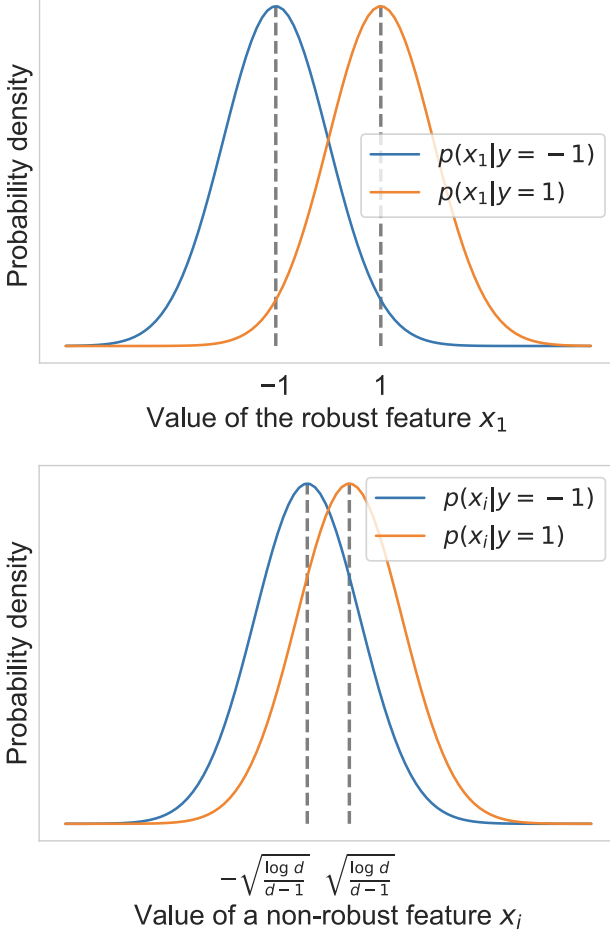
\includegraphics[width=0.5\columnwidth]{figures/adversarial_example.png}
% \end{wrapfigure}

$x\in\mathbb{R}^{d},y\sim{{Bernoulli}}(\{-1,1\}),Z_{i}\sim{\mathcal{N}}(0,1)$

- Robust features: $x_{1}=y+Z_{1}$

- Non-robust features: $x_{i}=y{\sqrt{\frac{\log d}{d-1}}}+Z_{i}, \; \forall i \in \{-1, 1\}$

- $d\to\infty \Rightarrow \ \uparrow$ adversarial risk and $\downarrow$ standard risk 

- using the robust feature $x_1$:

MLE: $\arg\operatorname*{max}_{\hat{y}\in\{\pm1\}}p(\hat{y}\;\vert\;x_{1})
=\\\operatorname*{arg}\operatorname*{max}_{{\hat{y}}\in\{\pm1\}}{\frac{p(x_{1}\mid{\hat{y}})p({\hat{y}})}{p(x_{1})}}
=\operatorname*{arg}\operatorname*{max}_{{\hat{y}}\in\{\pm1\}}{p(x_{1}\mid{\hat{y}})}$ 
assuming $p(y=1)=p(y=-1)$

- Standard Risk: $\int_{0}^{\infty}{\frac{1}{\sqrt{2\pi}}}e^{-0.5(x+1)^{2}}d x\approx0.16$ good but not perfect!

- using both robust and non-robust features:

MLE for all features $x_{i}=y a_{i}+Z_{i}$

$\arg\operatorname*{max}_{{\hat{y}}\in\{\pm1\}}p({\hat{y}}\mid x)$

$=\arg\operatorname*{max}_{{\hat{y}}\in\{\pm1\}}\prod_{i=1}^{d}p(x_{i}\mid{\hat{y}})$

$=\arg\operatorname*{max}_{{\hat{y}}\in\{\pm1\}}\sum_{i=1}^{d}\log p(x_{i}\mid{\hat{y}})$

$=\arg\operatorname*{max}_{{\hat{y}}\in\{\pm1\}}\sum_{i=1}^{d}\log \frac{1}{\sqrt{2\pi}}e^{-\frac{1}{2}(x_{i}-\hat{y}a_{i})^{2}}$

$=\arg\operatorname*{min}_{{\hat{y}}\in\{\pm1\}}\sum_{i=1}^{d}(x_{i}-\hat{y}a_{i})^{2}$

$=\arg\operatorname*{min}_{{\hat{y}}\in\{\pm1\}}\sum_{i=1}^{d}(x_{i}^{2}-2x_{i}\hat{y}a_{i}+\hat{y}^{2}a_{i}^{2})$

$=\arg\operatorname*{max}_{\hat{y}\in\{\pm1\}}{\hat{y}}\sum_{i=1}^{d}x_{i}a_{i}$

${\hat{y}}\sum_{i=1}^{d}x_{i}a_{i}=\hat{y}y(\sum_{i=1}^{d}a_{i}^{2})+\hat{y}\sum_{i=1}^{d}a_{i}Z_{i}=\hat{y}y(1+\log(d))+\hat{y}Z$ where $Z:=\textstyle\sum_{i=1}^{d}a_{i}Z_{i}\sim{\mathcal{N}}(0,1+\log d)$

Scaling by $1/(1+\log d)$ the MLE results in:

$y{\hat{y}}+{\hat{y}}Z\operatorname{with}Z\sim{\mathcal{N}}(0,1/(1+\log d))$

$d\rightarrow\infty,{\hat{y}}Z\rightarrow0 \Rightarrow$ standard risk $R(f) \rightarrow 0$ 

- using the non-robust features improves standard risk!

- Adversarial risk:

The adversary can use tiny $\ell_\infty$ perturbations:

$\varepsilon=2\sqrt{\frac{\log d}{d-1}}\,(\to0\,\mathrm{when})\,d\to\infty)$

${\hat{x}}_{1}=\left(1-2\sqrt{\frac{\log d}{d-1}}\right)y+Z_{1}$, almost unaffected

$\hat{x}_{i}=-\sqrt{\frac{\log d}{d-1}}y+Z_{i}$, completely flipped

$R_{\varepsilon}(f) \approx 1 \Rightarrow$ tradeoff between accuracy and robustness.

\sectiondivider

\sectionnewcolor
\section{Matrix Factorization}

Given items (movies) $d=1, 2, . . . , D$ and users $n= 1, 2, . . . , N$, we define X to be the $D \times N$ matrix containing all rating entries. That is, $x_{dn}$ is the rating of n-th user for d-th item.
Note that most ratings $x_{dn}$ are missing, and our task is to predict them accurately.

\subsection*{Algorithm}

$X \approx WZ^T$, $W \in \mathbb{R}^{D \times K}, \ Z \in \mathbb{R}^{N \times K}$ tall matrices $K << N, D$

$\operatorname*{min}_{W,Z}~{\mathcal{L}}(W,Z):=\frac{1}{2}\sum_{(d,n)\in\mathbb{Q}} [x_{dn}-(WZ^T)_{dn}]^2$

- We hope to ``explain" each rating $x_{dn}$ by a numerical representation of the corresponding item and user - in fact by the inner product of an item feature vector with the user feature vector.



- The set $\Omega\subseteq\left[D\right]\times\left[N\right]$ collects the indices of the observed ratings of the input matrix $X$.

- This cost is not jointly convex w.r.t. W and Z, nor identifiable as $(w^*, z^*) \Leftrightarrow (\beta w^*, \beta^{-1} z^*)$

\subsection*{Choosing K}

- $\uparrow K \Rightarrow$ overfitting ($\Leftrightarrow \ \downarrow K \Rightarrow$ underfitting). 
For $K >> N,D \Rightarrow (W^*, Z^{*^T}) = (X, I) = (I, X)$

\subsection*{Regularization}

$\frac{1}{2}\sum_{(d,n)\in\Omega}[x_{d n}-(W Z^{T})_{d n}]^{2}+\frac{\lambda_{w}}{2}||{W}||_{\mathrm{Frob}}^{2}+\frac{\lambda_{z}}{2}||{Z}||_{\mathrm{Frob}}^{2}$
$\lambda_{w},\lambda_{z}\, \in \mathbb{R} > 0$


\subsection*{Stochastic Gradient Descent}

$\mathcal{L} = \frac{1}{|\Omega|} \sum_{(d,n)\in\Omega}\underbrace{{\frac{1}{2}}[x_{d n}-(\mathbf{W}\mathbf{Z}^{\textsf{T}})_{d n}]^{2}}_{f_{d,n}}$

For one fixed element (d, n) of the sum, we derive the gradient entry (d', k) for W:

${\frac{\partial}{\partial w_{d^{\prime},k}}}f_{d,n}(W, Z) \in \mathbb{R}^{D\times K}=\\\left\{\begin{array}{l l}{-\left[x_{d n}-({\bf W Z}^{T})_{d n}\right]z_{n,k}\;\;\;\mathrm{if}\;d^{\prime}=d} \\ {0 \mathrm{~otherwise}}\end{array}\right.$

${\frac{\partial}{\partial z_{n^{\prime},k}}}f_{d,n}(W, Z)\in \mathbb{R}^{N\times K}=\\\left\{\begin{array}{l l}{-\left[x_{d n}-({\bf W Z}^{T})_{d n}\right]w_{d,k}\;\;\;\mathrm{if}\;n^{\prime}=n} \\ {0 \mathrm{~otherwise}}\end{array}\right.$

- cost: $\Theta(K)$ which is cheap!

\subsection*{Alternating Least Squares}

- No missing entries:

${\textstyle\frac{1}{2}}\sum_{d=1}^{D}\sum_{n=1}^{N}\left[x_{d n}-\left(W\mathbf{Z}^{\mathsf{T}}\right)_{d n}\right]^{2}$
$\\=\frac{1}{2}\|\mathbf{X}-\mathbf{W}\mathbf{Z}^{\mathsf{T}}\|_{{Frob}}^{2}$

- We first minimize w.r.t. Z for fixed W and then minimize W given Z (closed form solutions):

$Z^{\mathsf{T}}:=(\mathsf{W}^{\mathsf{T}}\mathsf{W}+\lambda_{z}\mathsf{I}_{K})^{-1}\mathsf{W}^{\mathsf{T}}\mathsf{X}$

$\mathbf{W}^{\mathsf{T}}:=(\mathbf{Z}^{\mathsf{T}}\mathbf{Z}+\lambda_{w}\mathbf{I}_{K})^{-1}\mathbf{Z}^{\mathsf{T}}\mathbf{X}^{\mathsf{T}}$

- Cost: need to invert a $K \times K$ matrix

- With missing entries:
Can you derive the ALS updates for the more general setting, when only the ratings $(d, n) \in \Omega$ contribute to the cost, i.e.
$\frac{1}{2}\sum_{(d,n)\in\Omega}\big[x_{d n}-\big(\mathsf{W Z}^{\mathsf{T}}\big)_{d n}\big]^{2}$

Compute the gradient with respect to each group of variables, and set to zero.

% \subsection*{Update for $Z$ with fixed $W$:}
% The ALS update for $Z^{\mathsf{T}}$ is given by:
% \[
% Z^{\mathsf{T}} := \left(W^{\mathsf{T}}W + \lambda_{z}I_{K}\right)^{-1}W^{\mathsf{T}}X
% \]
% For each $(n, k)$ where $(d', n) \in \Omega$, the update for the $k$-th component of $Z^{\mathsf{T}}$ is:
% \[
% \left(Z^{\mathsf{T}}\right)_{n,k} := \left(\sum_{d':(d',n)\in\Omega} w_{d',k'}w_{d',k} + \lambda_{z}\delta_{k,k'}\right)^{-1} \sum_{d':(d',n)\in\Omega} w_{d',k'}x_{d',n}
% \]

% \subsection*{Update for $W$ with fixed $Z$:}
% The ALS update for $W^{\mathsf{T}}$ is given by:
% \[
% W^{\mathsf{T}} := \left(Z^{\mathsf{T}}Z + \lambda_{w}I_{K}\right)^{-1}Z^{\mathsf{T}}X^{\mathsf{T}}
% \]
% For each $(d, k)$ where $(d, n') \in \Omega$, the update for the $k$-th component of $W^{\mathsf{T}}$ is:
% \[
% \left(W^{\mathsf{T}}\right)_{d,k} := \left(\sum_{n':(d,n')\in\Omega} z_{n',k'}z_{n',k} + \lambda_{w}\delta_{k,k'}\right)^{-1} \sum_{n':(d,n')\in\Omega} z_{n',k'}x_{d,n'}
% \]

\sectiondivider

\sectionnewcolor
\section*{Text Representation}

-Finding numerical representations for words is fundamental for all machine learning methods dealing with text data.

-Goal: For each word, find mapping (embedding) $w_{i} \mapsto \mathbf{w}_{i} \in \mathbb{R}^{K}$

\subsection*{Co-Occurence Matrix}

-A big corpus of un-labeled text can be represented as the co-occurrence counts. $n_{i j}:=$ \#contexts where word $w_{i}$ occurs together with word $w_{j}$.

- Needs definition of Context e.g. document, paragraph, sentence, window and Vocabulary $\mathcal{V}:=\left\{w_{1}, \ldots, w_{D}\right\}$

- For words $w_{d}=1,2, \ldots, D$ and context words $w_{n}=1,2, \ldots, N$, the co-occurence counts $n_{i j}$ form a very sparse $D \times N$ matrix.

\subsection*{Learning Word-Representations}

- Find a factorization of the cooccurence matrix!

- Typically uses $\log$ of the actual counts, i.e. $x_{d n}:=\log \left(n_{d n}\right)$.

- Aim to find $\mathbf{W}, \mathbf{Z}$ s.t. $
\mathbf{X} \approx \mathbf{W} \mathbf{Z}^{\top}
$

$
\min _{\mathbf{W}, \mathbf{Z}} \mathcal{L}(\mathbf{W}, \mathbf{Z}):=\\\frac{1}{2} \sum_{(d, n) \in \Omega} f_{d n}\left[x_{d n}-\left(\mathbf{W} \mathbf{Z}^{\top}\right) d n\right]^{2}
$

where $\mathbf{W} \in \mathbb{R}^{D \times K}$, $\mathbf{Z} \in \mathbb{R}^{N \times K}$, $K \ll$ $D, N$, $\Omega \subseteq[D] \times[N]$ indices of non-zeros of the count matrix $\mathbf{X}$, $f_{d n}$ are weights to each entry.

\subsection*{GloVe}
A variant of word2vec.

$f_{d n}:=\min \left\{1,\left(n_{d n} / n_{\max }\right)^{\alpha}\right\}, \quad \alpha \in[0 ; 1] \quad$ (e.g. $\alpha=\frac{3}{4}$)

\textbf{Note:} Choosing K; $K$ e.g. 50, 100, 500

\subsection*{Training}
- Stochastic Gradient Descent (SGD) ($\Theta(K)$ per step $\rightarrow$ easily parralelizable)

- Alternating Least-Squares (ALS)

\subsection*{Skip-Gram Model}
- Uses binary classification (logistic regression objective), to separate real word pairs $\left(w_{d}, w_{n}\right)$ from fake word pairs. Same inner product score $=$ matrix factorization.

- Given $w_{d}$, a context word $w_{n}$ is:

real $=$ appearing together in a context window of size 5

fake $=$ any word $w_{n^{\prime}}$ sampled randomly: Negative sampling (also: Noise Contrastive Estimation)

\section*{Learning Representations of Sentences \& Documents}
- Supervised: For a supervised task (e.g. predicting the emotion of a tweet), we can use matrix factorization or CNNs.
- Unsupervised: 

Adding or averaging (fixed, given) word vectors, 

Training word vectors such that adding/averaging works well

Direct unsupervised training for sentences (appearing together with context sentences) instead of words

\subsection*{Fast Text}
Matrix factorization to learn document/sentence representations (supervised).

Given a sentence $s_{n}=$ $\left(w_{1}, w_{2}, \ldots, w_{m}\right)$, let $\mathbf{x}_{n} \in \mathbb{R}^{|\mathcal{V}|}$ be the bag-of-words representation of the sentence.

$$
\min _{\mathbf{W}, \mathbf{Z}} \mathcal{L}(\mathbf{W}, \mathbf{Z}):=\sum_{s_{n} \text { a sentence }} f\left(y_{n} \mathbf{W} \mathbf{Z}^{\top} \mathbf{x}_{n}\right)
$$

where $\mathbf{W} \in \mathbb{R}^{1 \times K}, \mathbf{Z} \in \mathbb{R}^{|\mathcal{V}| \times K}$ are the variables, and the vector $\mathbf{x}_{n} \in \mathbb{R}^{|\mathcal{V}|}$ represents our $n$-th training sentence.

Here $f$ is a linear classifier loss function, and $y_{n} \in\{ \pm 1\}$ is the classification label for sentence $\mathbf{x}_{n}$.


\subsection*{Language Models}
\subsubsection*{Selfsupervised training:}
- Can a model generate text? train classifier to predict the continuation (next word) of given text

- Multi-class:
Use soft-max loss function with a large number of classes $D=$ vocabulary size

- Binary classification: 
Predict if next word is real or fake (i.e. as in word2vec)

- Impressive recent progress using large models, such as transformers

\sectiondivider

\sectionnewcolor
\newpage
\section{{\textcolor[RGB]{255,0,0}{This is RGB red text.}}}

For $x \in[r_{i-1},r_{i}]$ \\
$r(x)={\tilde{a}}_{1}x+{\tilde{b}}_{1}+\sum_{j=2}^{m}{\tilde{a}}_{j}(x-{\tilde{b}}_{j})_{+}$

\hrulefill

$\begin{array}{l}{{\mathsf{For}\;x\in[r_{i-1},r_{i}]}}\\ {{r(x)={\tilde{a}}_{1}x+{\tilde{b}}_{1}+\sum_{j=2}^{m}{\tilde{a}}_{j}(x-{\tilde{b}}_{j})_{+}}}\end{array}$\\
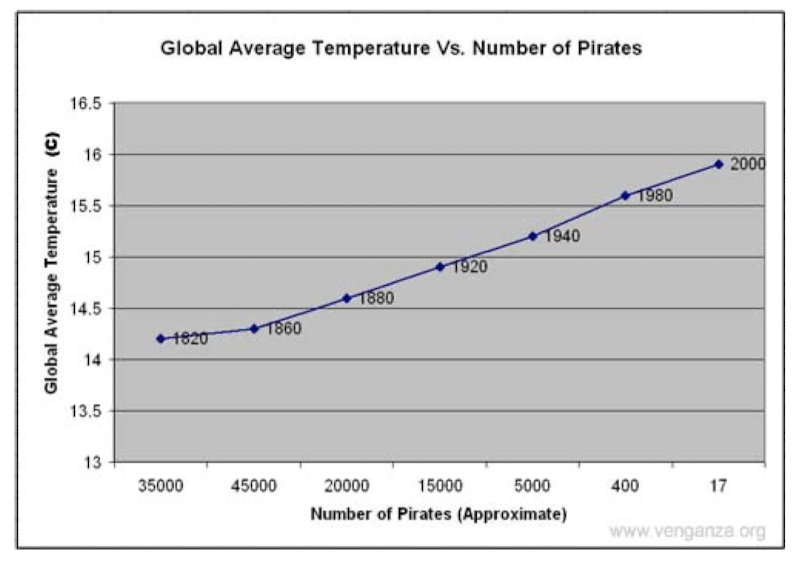
\includegraphics[width=\linewidth]{test_image}

\lipsum[1]

\noindent\dotfill

\lipsum[1]
\sectiondivider

\end{multicols*}

\end{document}
